% !TEX root = widefieldscan.tex
\svnidlong
{$HeadURL$}
{$LastChangedDate$}
{$LastChangedRevision$}
{$LastChangedBy$}
%
\section{Discussion}\label{sec:Discussion}

We present a method to laterally increase the field of view of tomographic imaging systems operated in parallel beam geometry and would like to call this method wide field synchrotron radiation based x-ray tomographic microscopy (WF-SRXTM). We selectively defined different scanning protocols for the optimization of the total imaging time towards the expected imaging quality. This enables a very fast acquisition of lower quality tomographic datasets, or acquisition of very high quality datasets in a longer time. Even if the reduction in scanning time does introduce artifacts in the three-dimensional reconstruction, as specified in section~\ref{subsec:comparison}, an automated segmentation of the airway segments in the sample is still possible, even for the protocol with greatly reduced scanning time.

Reducing the scanning time by \SI{84}{\percent} compared to an unoptimized gold standard scan, also greatly reduces radiation dose inflicted on the sample. For this publication, the radiation dose inflicted on the sample was of secondary concern, since our sample was embedded in paraffin and was not used for further investigations. Nonetheless, such a reduction in radiation dose is the first step to in vivo measurements at TOMCAT. Irradiating living organisms for a prolonged time is neither feasible nor desired, especially if biological development is studied, which require multiple exposures of the same individual over a prolonged time-frame. Reducing the radiation dose by \SI{84}{\percent} with a suitable protocol makes WF-SRXTM an option for ultra high-resolution images of in vivo processes with enhanced field of view.

The field of view was increased three-fold by merging projections from three subscans and reconstructing these merged projections using the standard workflow at the TOMCAT beamline~\cite{Hintermueller2009}. As a consequence of increasing the field of view, an increased amount of projections had to be acquired to satisfy the sampling theorem. This increased amount of projections lengthened the acquisition time. To overcome this limitation, we defined multiple scanning protocols with a reduced amount of total projections and thus reduced acquisition time and thus reduced radiation dose. All these protocols were evaluated for quality of the resulting reconstructions compared to a gold standard. We have shown that the resulting quality can be simulated prior to scanning, thus giving the end-user a possibility to chose a suited scanning protocol, based on the demands for scanning time optimization and quality of the resulting tomographic dataset.

Reducing the amount of projections for the central of the three subscans obviously led to a decrease in scanning quality when compared to a gold-standard scan, albeit we postulate that such a reduction can be performed without loss of fidelity in the resulting reconstructions (compare e.g.\  protocols B and C or D and E, where the amount of projections for the central subscan has been halved in comparison to the outer subscans. In both cases we reduce the scanning time by approximately 2500 projections, but also reduce the quality of the scans by approximately \SI{20}{\percent}.

In contrast to this finding, we see that a reduction of the number of projections for the central of the three subscans leads to a decreased quality of the scan. We studied this in more details with additional datasets which have been artificially generated. Those datasets have been scanned with an equal amount of projections for each subscan. Additional artificial central subscans have been generated with half the amount of projections. This has been done to eradicate possible alignment errors of the beamline. We scanned four protocols (A, B, C and D, details see table~\ref{tab:abcd}) and artificially reduced the amount of projections of the central subscan prior to reconstruction. 

\begin{table}
	\centering
	\caption{Details of the protocols with artificially reduced amount of projections for the central scan to simulate influence of merging and interpolation.}
	% Table generated by Excel2LaTeX from sheet 'Sheet1'
	\begin{tabular}{lcccclccc}
		Protocol & $\textrm{s}_{1}$ & $\textrm{s}_{2}$ & $\textrm{s}_{3}$ &  &  Protocol & $\textrm{s}_{1}$ & $\textrm{s}_{2}$ & $\textrm{s}_{3}$ \\
		A & 5040 & 5040 & 5040 &  &  B & 4536 & 4536 & 4536 \\
		A$\frac{\textrm{Central}}{2}$ & 5040 & 2520 & 5040 &  & B$\frac{\textrm{Central}}{2}$ & 4536 & 2268 & 4536 \\
		A$\frac{\textrm{Central}}{4}$ & 5040 & 1260 & 5040 &  & B$\frac{\textrm{Central}}{4}$ & 4536 & 1134 & 4536 \\
		A$\frac{\textrm{Central}}{8}$ & 5040 & 630 & 5040 &  & B$\frac{\textrm{Central}}{8}$ & 4536 & 567 & 4536 \\
		\hline
		C & 4032 & 4032 & 4032 &  &  D & 3528 & 3528 & 3528 \\
		C$\frac{\textrm{Central}}{2}$ & 4032 & 2016 & 4032 &  & D$\frac{\textrm{Central}}{2}$ & 3528 & 1764 & 3528 \\
		C$\frac{\textrm{Central}}{4}$ & 4032 & 1008 & 4032 &  & D$\frac{\textrm{Central}}{4}$ & 3528 & 882 & 3528 \\
		C$\frac{\textrm{Central}}{8}$ & 4032 & 504 & 4032 &  & D$\frac{\textrm{Central}}{8}$ & 3528 & 441 & 3528 \\
	\end{tabular}  
	\label{tab:abcd}
\end{table}

After reconstruction, we assessed the structural similarity index \cite{Wang2004} of multiple slices in comparison to the protocol with the maximal amount of acquired projections for this experiment (A)\footnote{The normalized error (as shown in figure~\ref{fig:NormalizedErrorPlot}) has also been calculated and shows the same result.}). As can be seen in figure~\ref{fig:ssimplot}, the structural similarity index (SSIM) greatly decreases for a reduced amount of projections of the central subscan. Halving the projections of the central subscan reduces the SSIM for protocol A$\frac{\textrm{Central}}{2}$ (12600 total projections) lower than the quality of the unreduced protocol C (12096 total projections). Reducing the central subscan down to 630 projections (A$\frac{\textrm{Central}}{8}$, 10710 total projections), the quality of the reconstructions drops to the quality of the unreduced scan D (total 10584 projections). 

\begin{figure}
	\centering
		\caption{Plots of the mean SSIM parameter for 18 slices for each of the protocols with artificially reduced central subscans}
	\ifiucr		
		% This file was created by matlab2tikz v0.0.4.
%\documentclass{article}
%\usepackage{tikz,pgfplots,lipsum}
%\usepackage[pdftex,active,tightpage]{preview}
%\begin{document}
%\begin{preview}
%%%%%%%%%%%%
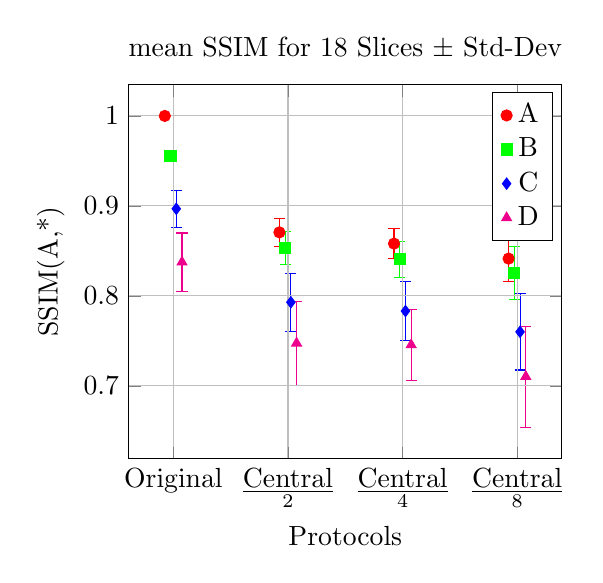
\begin{tikzpicture}

% Axis at [0.13 0.11 0.78 0.81]
\begin{axis}[
xmajorgrids,xminorgrids,
ymajorgrids,yminorgrids,
axis on top,
scale only axis,
width=5.5cm,
%height=3.56562in,
%xmin=0.5, xmax=4.5,
%ymin=0.65, ymax=1,
xtick={1,2,3,4},
xticklabels={Original,%
	$\frac{\textrm{Central}}{2}$,%
	$\frac{\textrm{Central}}{4}$,%
	$\frac{\textrm{Central}}{8}$},
xlabel={Protocols},
ylabel={SSIM(A,*)},
title={mean SSIM for 18 Slices $\pm$ Std-Dev},
legend entries={A,B,C,D}
]

\addplot [ color=red, only marks, mark=*]
plot[error bars/.cd, y dir = both, y explicit]
coordinates{
 (0.925,1) +- (0,0)
 (1.925,0.870644) +- (0,0.0155253)
 (2.925,0.85813) +- (0,0.0163216)
 (3.925,0.841459) +- (0,0.0251378)
};

\addplot [ color=green, solid, only marks, mark=square*]
plot[error bars/.cd, y dir = both, y explicit]
coordinates{
 (0.975,0.955859) +- (0,0.00451414)
 (1.975,0.853525) +- (0,0.0184261)
 (2.975,0.840652) +- (0,0.0198974)
 (3.975,0.825281) +- (0,0.0293097)
};

\addplot [ color=blue, solid, only marks, mark=diamond*]
plot[error bars/.cd, y dir = both, y explicit]
coordinates{
 (1.025,0.896816) +- (0,0.0204368)
 (2.025,0.79298) +- (0,0.0322583)
 (3.025,0.78324) +- (0,0.032939)
 (4.025,0.760095) +- (0,0.0424208)
};

\addplot [ color=magenta, solid, only marks, mark=triangle*]
plot[error bars/.cd, y dir = both, y explicit]
coordinates{
 (1.075,0.837564) +- (0,0.0323791)
 (2.075,0.74749) +- (0,0.0465387)
 (3.075,0.745587) +- (0,0.0392654)
 (4.075,0.710318) +- (0,0.056185)
};

\end{axis}

\end{tikzpicture}
%%%%%%%%%%%%
%\end{preview}
%\end{document}%
	\else
	\fi
	\label{fig:ssimplot}
\end{figure}

\renewcommand{\imsize}{.245\columnwidth}
\begin{figure}
	\centering
	\caption{Details of the protocols with artificially reduced central subscans. Crop to the central part of the tomographic reconstruction, 512 pixels wide. Visible ripples are introduced for protocols Ab and Ac through the strong undersampling of the central subscan.}
	\ifiucr
		\pgfmathsetlength{\imagewidth}{\imsize}%
		\pgfmathsetlength{\imagescale}{\imagewidth/512}%
		\begin{tikzpicture}[x=\imagescale,y=-\imagescale]
			\def\x{316} % scalebar-x at golden ratio of x=512px
			\def\y{461} % scalebar-y at 90% of height of y=512px
			\node[anchor=north west,inner sep=0pt,outer sep=0pt] at (0,0)
	    		{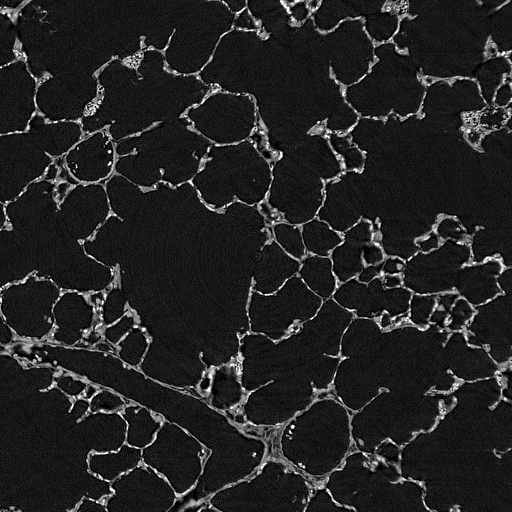
\includegraphics[width=\imagewidth]{img/ripples/R108C36B-A-mrg1024_rec_8bit.png}};
			% 513px = 0.75776mm > 100px = 148um > 338px = 500um, 68px = 100um
			%\draw[color=white,|-|,thick] (0,118) -- (512,117) node [sloped,midway,above] {\SI{0.75776}{\milli\meter} (512px)};
			\draw[color=white,|-|,thick] (\x,\y) -- (\x+136,\y) node [midway,above] {\SI{200}{\micro\meter}};
			\node [color=white,anchor=south west] at (0,512) {A};
		\end{tikzpicture}%
		\hfill%
		\begin{tikzpicture}[x=\imagescale,y=-\imagescale]
			\def\x{316} % scalebar-x at golden ratio of x=512px
			\def\y{461} % scalebar-y at 90% of height of y=512px
			\node[anchor=north west,inner sep=0pt,outer sep=0pt] at (0,0)
	    		{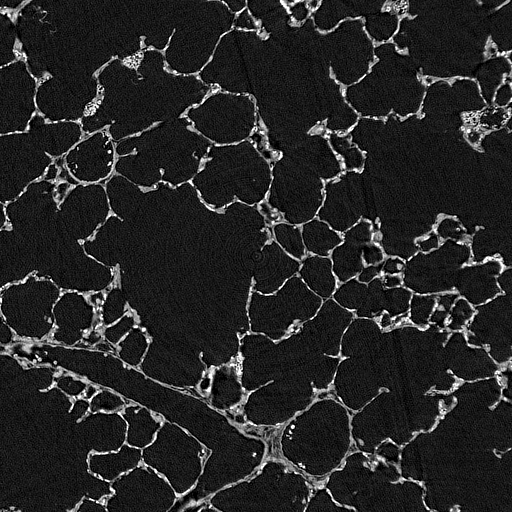
\includegraphics[width=\imagewidth]{img/ripples/R108C36B-Aa-mrg1024_rec_8bit.png}};
			% 513px = 0.75776mm > 100px = 148um > 338px = 500um, 68px = 100um
			%\draw[color=white,|-|,thick] (0,118) -- (512,117) node [sloped,midway,above] {\SI{0.75776}{\milli\meter} (512px)};
			\draw[color=white,|-|,thick] (\x,\y) -- (\x+136,\y) node [midway,above] {\SI{200}{\micro\meter}};
			\node [color=white,anchor=south west] at (0,512) {Aa};
		\end{tikzpicture}%
		\hfill%
		\begin{tikzpicture}[x=\imagescale,y=-\imagescale]
			\def\x{316} % scalebar-x at golden ratio of x=512px
			\def\y{461} % scalebar-y at 90% of height of y=512px
			\node[anchor=north west,inner sep=0pt,outer sep=0pt] at (0,0)
	    		{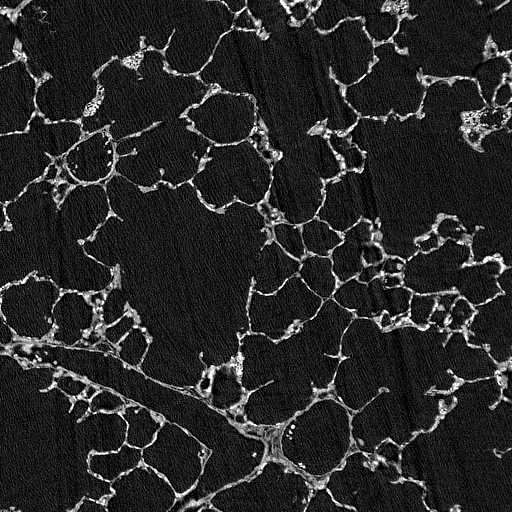
\includegraphics[width=\imagewidth]{img/ripples/R108C36B-Ab-mrg1024_rec_8bit.png}};
			% 513px = 0.75776mm > 100px = 148um > 338px = 500um, 68px = 100um
			%\draw[color=white,|-|,thick] (0,118) -- (512,117) node [sloped,midway,above] {\SI{0.75776}{\milli\meter} (512px)};
			\draw[color=white,|-|,thick] (\x,\y) -- (\x+136,\y) node [midway,above] {\SI{200}{\micro\meter}};
			\node [color=white,anchor=south west] at (0,512) {Ab};
		\end{tikzpicture}%
		\hfill%
		\begin{tikzpicture}[x=\imagescale,y=-\imagescale]
			\def\x{316} % scalebar-x at golden ratio of x=512px
			\def\y{461} % scalebar-y at 90% of height of y=512px
			\node[anchor=north west,inner sep=0pt,outer sep=0pt] at (0,0)
	    		{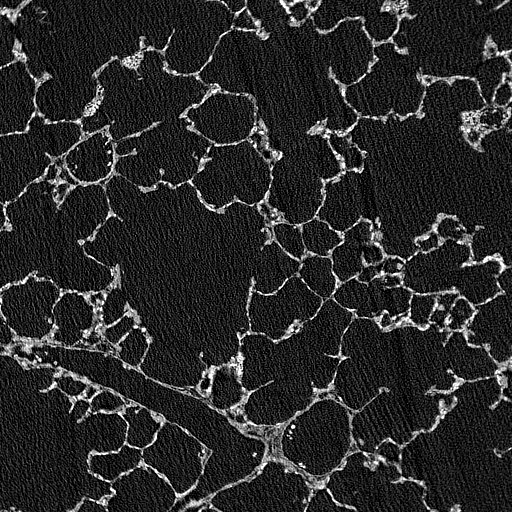
\includegraphics[width=\imagewidth]{img/ripples/R108C36B-Ac-mrg1024_rec_8bit.png}};
			% 513px = 0.75776mm > 100px = 148um > 338px = 500um, 68px = 100um
			%\draw[color=white,|-|,thick] (0,118) -- (512,117) node [sloped,midway,above] {\SI{0.75776}{\milli\meter} (512px)};
			\draw[color=white,|-|,thick] (\x,\y) -- (\x+136,\y) node [midway,above] {\SI{200}{\micro\meter}};
			\draw[color=white,anchor=south west] (0,512) node {Ac};
		\end{tikzpicture}%
	\else
	\fi	
	\label{fig:ssim-details}
\end{figure}

We postulate that the interpolation of the missing projections introduces errors in the resulting reconstruction, leading to a decreased quality. Additionally---when taking the SSIM into account---the quality of the reconstructions scales with the total amount of projections acquired for all subscans. We thus include only such protocols where the amount of projections of the central subscan is halved in comparison to the outer subscans for the end-user to choose from.

For protocols with an equal amount of total projections, but differing numbers of projections for the central and ring scans we observed a difference in reconstruction quality. Protocols C and D as well as protocols M and N are such protocols and are marked in figure~\ref{fig:NormalizedErrorPlot}. Please refer to table~\ref{tab:protocols} for details of these four protocols. This makes it necessary to interpolate projections for the central subscans for both protocol C and M, which decreases the quality of the scan. Additionally, for protocols D and N, the central subscan is oversampled, which does not significantly contribute to the quality of the reconstructions, but makes additional scanning projections necessary. 

The quality $E_{i_{norm}}$ of protocols C and D are not significantly different, and the quality of protocols M and N is closely comparable. As a consequence, it thus seems desirable to favor a protocol where the central scan is not oversampled, when being able to choose two protocols with the exact same amount of total projections. Even if this introduces additional computing time for interpolating projections prior to reconstruction, these protocols show an increased quality compared to protocols where the central scan is oversampled. Since an oversampling of the central scan does not add to the total reconstruction quality, this explanation seems natural. Such greatly oversampled protocols are also excluded from the protocols which the end-user chooses from.

We have shown that the field of view of parallel beam tomographic end-stations can be increased up to five-fold and have three-dimensionally reconstructed multiple tomograms obtained with WF-SRXTM. The protocols are theoretically expandable for more than the shown 5 subscans, although the reconstruction of wide field scans with 7 or more subscans places tremendous requirements on the data processing infrastructure. The datasets shown in figure~\ref{fig:BvsT} are binned scans resulting in datasets of 1024 slices, each with a size of 2792$\times$2792 pixels at a \SI{8}{\bit} depth. This amounts to a total size of the dataset of approximately \SI{7.5}{\giga\byte}. If we assume an un-binned scan with 7 overlapping subscans, the size of the stitched projections will be around 14000$\times$14000 pixels. The full dataset will consist of 2048 stitched slices with that size, which amounts to a total size of approximately \SI{383}{\giga\byte} for the full dataset. All datasets referred to were reconstructed at \SI{8}{\bit}, while TOMCAT also offers the possibility to obtain tomographic datasets with \SI{16}{\bit} depth. A wide field scan with a seven-fold increase in field of view with increased bit depth would result in one dataset with a size of \SI{0.75}{\tera\byte}.

Even if the amount of data to handle is humongous, a wide field scan with a five-fold increase in field of view remains interesting, since it would enable the end-user to selectively reconstruct regions of interest from large samples with ultra-high resolution. Up to now, a two-step process was required to scan such regions from samples larger than the field of view with high resolutions. In a first step, a registered overview scan of the sample at lower resolution, and thus large field of view, was acquired. Then a region of interest to be scanned with high resolution was defined and marked in the low-resolution dataset, using a custom-made ROI picker software~\cite{Heinzer2008}, and a high resolution local tomography scan, with small field of view, was performed at the marked region.

One disadvantage of WF-SRXTM compared with the ROI picker method, are the extremely big datasets that result from the reconstruction of the full resolution projections into reconstructions spanning a large field of view. With the ROI picker method, only selective regions of interest, selected from a low-resolution tomogram, are scanned and reconstructed in high resolution, thus reducing the amount of data recorded. Since we record all data in a one-step process, it would be possible to integrate partial reconstructions of the full size datasets into the data processing pipeline of TOMCAT. After definition of a ROI to be reconstructed out of the high-resolution wide field dataset, partial sinograms and partial reconstructions could be calculated, avoiding a two-step process. 